\documentclass[11pt,aspectratio=169]{beamer}

% Clean minimal theme
\usetheme{Boadilla}
\usefonttheme[onlymath]{serif}
\useinnertheme{circles}
\setbeamertemplate{navigation symbols}{}

\setbeamertemplate{footline}{%
  \leavevmode\hbox{%
    \begin{beamercolorbox}[wd=.33\paperwidth,ht=2.25ex,dp=1ex,center]{author in head/foot}%
      \usebeamerfont{author in head/foot}\insertshortauthor
    \end{beamercolorbox}%
    \begin{beamercolorbox}[wd=.34\paperwidth,ht=2.25ex,dp=1ex,center]{title in head/foot}%
      \usebeamerfont{title in head/foot}\insertshorttitle
    \end{beamercolorbox}%
    \begin{beamercolorbox}[wd=.33\paperwidth,ht=2.25ex,dp=1ex,right]{date in head/foot}%
      \usebeamerfont{date in head/foot}\insertframenumber{} / \inserttotalframenumber\hspace*{2ex}
    \end{beamercolorbox}%
  }\vskip0pt%
}

\usepackage[T1]{fontenc}
\usepackage[utf8]{inputenc}
\usepackage[scaled=0.92]{helvet}
\renewcommand{\familydefault}{\sfdefault}
\usepackage{amsmath,amssymb}
\usepackage{booktabs}
\usepackage{graphicx}
\usepackage{xcolor}
\usepackage{array}

\graphicspath{{../figures/}}

% Soft color palette
\definecolor{softnavy}{HTML}{2C3E50}
\definecolor{softteal}{HTML}{2980B9}
\definecolor{accentblue}{HTML}{2980B9}
\definecolor{accentred}{HTML}{E74C3C}
\definecolor{accentgreen}{HTML}{27AE60}
\definecolor{lightgray}{HTML}{ECF0F1}
\definecolor{warmgray}{HTML}{F4F6F7}
\definecolor{darktext}{HTML}{2C3E50}

% Beamer color scheme
\setbeamercolor{structure}{fg=softnavy}
\setbeamercolor{palette primary}{bg=softnavy,fg=white}
\setbeamercolor{palette secondary}{bg=softteal,fg=white}
\setbeamercolor{palette tertiary}{bg=softnavy,fg=white}
\setbeamercolor{frametitle}{fg=softnavy,bg=warmgray}
\setbeamercolor{title}{fg=softnavy}
\setbeamercolor{block title}{bg=softteal,fg=white}
\setbeamercolor{block body}{bg=lightgray,fg=darktext}
\setbeamercolor{item}{fg=softteal}
\setbeamercolor{normal text}{fg=darktext}
\setbeamercolor{author in head/foot}{bg=softnavy,fg=white}
\setbeamercolor{title in head/foot}{bg=softteal!80,fg=white}
\setbeamercolor{date in head/foot}{bg=softnavy!80,fg=white}

% Softer typography
\setbeamerfont{title}{series=\bfseries,size=\Large}
\setbeamerfont{frametitle}{series=\bfseries,size=\large}

\title[Math4AI Capstone]{From Linear Scores to a Single Hidden Layer}
\subtitle{A Mathematical Study of Simple Learning Systems}
\author[Feyzullayev, Samadov, Abdullazade]{Sharaf Feyzullayev \and Nijat Samadov \and Samir Abdullazade}
\institute{National AI Center --- AI Academy}
\date{Math4AI Final Capstone, April 2026}
\titlegraphic{\vspace{-0.5em}\includegraphics[width=4cm]{ai_academy_logo.png}}

\begin{document}

% ──────────────────────────────────────────
% SLIDE 1: Title
% ──────────────────────────────────────────
\begin{frame}
\titlepage
\end{frame}

% ──────────────────────────────────────────
% SLIDE 2: Central Question
% ──────────────────────────────────────────
\begin{frame}{The Central Question}

\begin{block}{Research Question}
\textit{When does a one-hidden-layer nonlinear classifier genuinely improve on a linear decision rule, and when is additional model complexity unnecessary?}
\end{block}

\vspace{0.6em}

\textbf{Our approach - argue from evidence, not preference:}
\begin{itemize}
    \item Compare \textbf{softmax regression} (linear baseline) against a \textbf{one-hidden-layer neural network} ($\tanh$ + softmax)
    \item Three datasets of increasing geometric complexity: Gaussian blobs, moons, digits
    \item Derive the mathematics that each model relies on, then test experimentally
    \item \textbf{More complexity is not automatically better}, if the linear baseline is sufficient, we say so and justify it
\end{itemize}
\end{frame}

% ──────────────────────────────────────────
% SLIDE 2b: Fair Comparison
% ──────────────────────────────────────────
\begin{frame}{Why the Comparison is Fair}

\textbf{Datasets}: 
\begin{itemize}
    \item \textbf{Linear Gaussian} ($n{=}400$), \textbf{Moons} ($n{=}400$)
    \item \textbf{Digits} ($n{=}1{,}797$, $d{=}64$, $K{=}10$)
\end{itemize}

\vspace{0.1em}
\begin{columns}[T]
\begin{column}{0.48\textwidth}
\textbf{Shared across models:}
\begin{itemize}
    \item \textbf{Train/Val/Test Split:} 60/20/20
    \item Preprocessing: Normalization only
    \item $L_2$ regularisation: $\lambda = 10^{-4}$
    \item Epoch budget: 200
    \item Mini-batch size: 64
\end{itemize}
\end{column}
\begin{column}{0.48\textwidth}
\textbf{Model selection protocol:}
\begin{itemize}
    \item Best checkpoint chosen on \textbf{validation CE only}
    \item Test set touched \textbf{exactly once} per seed
    \item 5 random seeds with 95\% CI reporting
\end{itemize}
\end{column}
\end{columns}

\end{frame}

% ──────────────────────────────────────────
% SLIDE 3: Models
% ──────────────────────────────────────────
\begin{frame}{Two Models, Same Objective}

\begin{columns}[T]
\begin{column}{0.48\textwidth}
\textbf{Model 1: Softmax Regression}
\[
s(x) = Wx + b
\]
\[
p_j(x) = \frac{\exp(s_j)}{\sum_\ell \exp(s_\ell)}
\]
\begin{itemize}
    \item \textbf{Geometry:} hyperplane boundaries
    \item 650 params on Digits ($Kd + K$)
    \item Represents exactly the family of affine classifiers
\end{itemize}
\end{column}

\begin{column}{0.48\textwidth}
\textbf{Model 2: One-Hidden-Layer NN}
\[
h = \tanh(W_1 x + b_1)
\]
\[
s = W_2 h + b_2
\]
\begin{itemize}
    \item \textbf{Geometry:} curved boundaries
    \item 2{,}410 params on Digits ($3.7\times$ more)
    \item Hidden layer = learned nonlinear coordinate change
\end{itemize}
\end{column}
\end{columns}

\vspace{0.5em}
\end{frame}

% ──────────────────────────────────────────
% SLIDE 3b: Objective Function
% ──────────────────────────────────────────
\begin{frame}{Objective: Negative Log-Likelihood}

Before optimizing, we define our loss function. Both models minimize the \textbf{Cross-Entropy (CE) Loss}, which is mathematically equivalent to the Negative Log-Likelihood for a categorical distribution:
\[
\mathcal{L} = -\frac{1}{n} \sum_{i=1}^n \log p_{y_i}(x_i)
\]

\begin{itemize}
    \item \textbf{Probabilistic meaning}: Maximizes the likelihood of the training data.
    \item \textbf{Optimization}: Provides clean, numerically stable gradients when paired with softmax.
\end{itemize}

\end{frame}

% ──────────────────────────────────────────
% SLIDE 4: Backpropagation
% ──────────────────────────────────────────
\begin{frame}{Backpropagation: Chain Rule in Action}

\textbf{Idea:} propagate loss sensitivities backward through the computation graph.

\vspace{0.3em}
\textbf{Key gradient formulas (vectorized):}
\begin{align*}
\frac{\partial \mathcal{L}}{\partial S} &= \tfrac{1}{n}(P - Y) \\[4pt]
\frac{\partial \mathcal{L}}{\partial W_2} &= \left(\tfrac{\partial \mathcal{L}}{\partial S}\right)^\top H \\[4pt]
\frac{\partial \mathcal{L}}{\partial Z_1} &= \tfrac{\partial \mathcal{L}}{\partial S}\, W_2 \odot (1 - H \odot H) \\[4pt]
\frac{\partial \mathcal{L}}{\partial W_1} &= \left(\tfrac{\partial \mathcal{L}}{\partial Z_1}\right)^\top X
\end{align*}

\end{frame}

% ──────────────────────────────────────────
% SLIDE 4b: Sanity Checks
% ──────────────────────────────────────────
\begin{frame}{Implementation Sanity Checks}

Before running experiments, we rigorously verified the from-scratch implementation:

\begin{table}[h]
    \centering
    \renewcommand{\arraystretch}{1.3} % Add some padding
    \begin{tabular}{@{}llc@{}}
        \toprule
        \textbf{Check} & \textbf{Result} & \textbf{Status} \\
        \midrule
        \textbf{Probability Normalization} & Softmax rows sum exactly to 1.0 & \textcolor{accentgreen}{Pass} \\
        \textbf{Monotonic Loss Decrease} & Loss strictly decreases ($1.62 \rightarrow 1.34$) & \textcolor{accentgreen}{Pass} \\
        \textbf{Numerical Gradient Check} & Max error $< 10^{-11}$ & \textcolor{accentgreen}{Pass} \\
        \textbf{No NaN/Inf Detection} & Parameters remain finite after training & \textcolor{accentgreen}{Pass} \\
        \textbf{Micro-dataset Overfit} & 10 samples fit to 100\% training accuracy & \textcolor{accentgreen}{Pass} \\
        \bottomrule
    \end{tabular}
\end{table}

\end{frame}

% ──────────────────────────────────────────
% SLIDE 5: Linear Gaussian
% ──────────────────────────────────────────
\begin{frame}{Experiment 1: Linear Gaussian --- Linear Model is Sufficient}

\begin{columns}[c]
\begin{column}{0.60\textwidth}
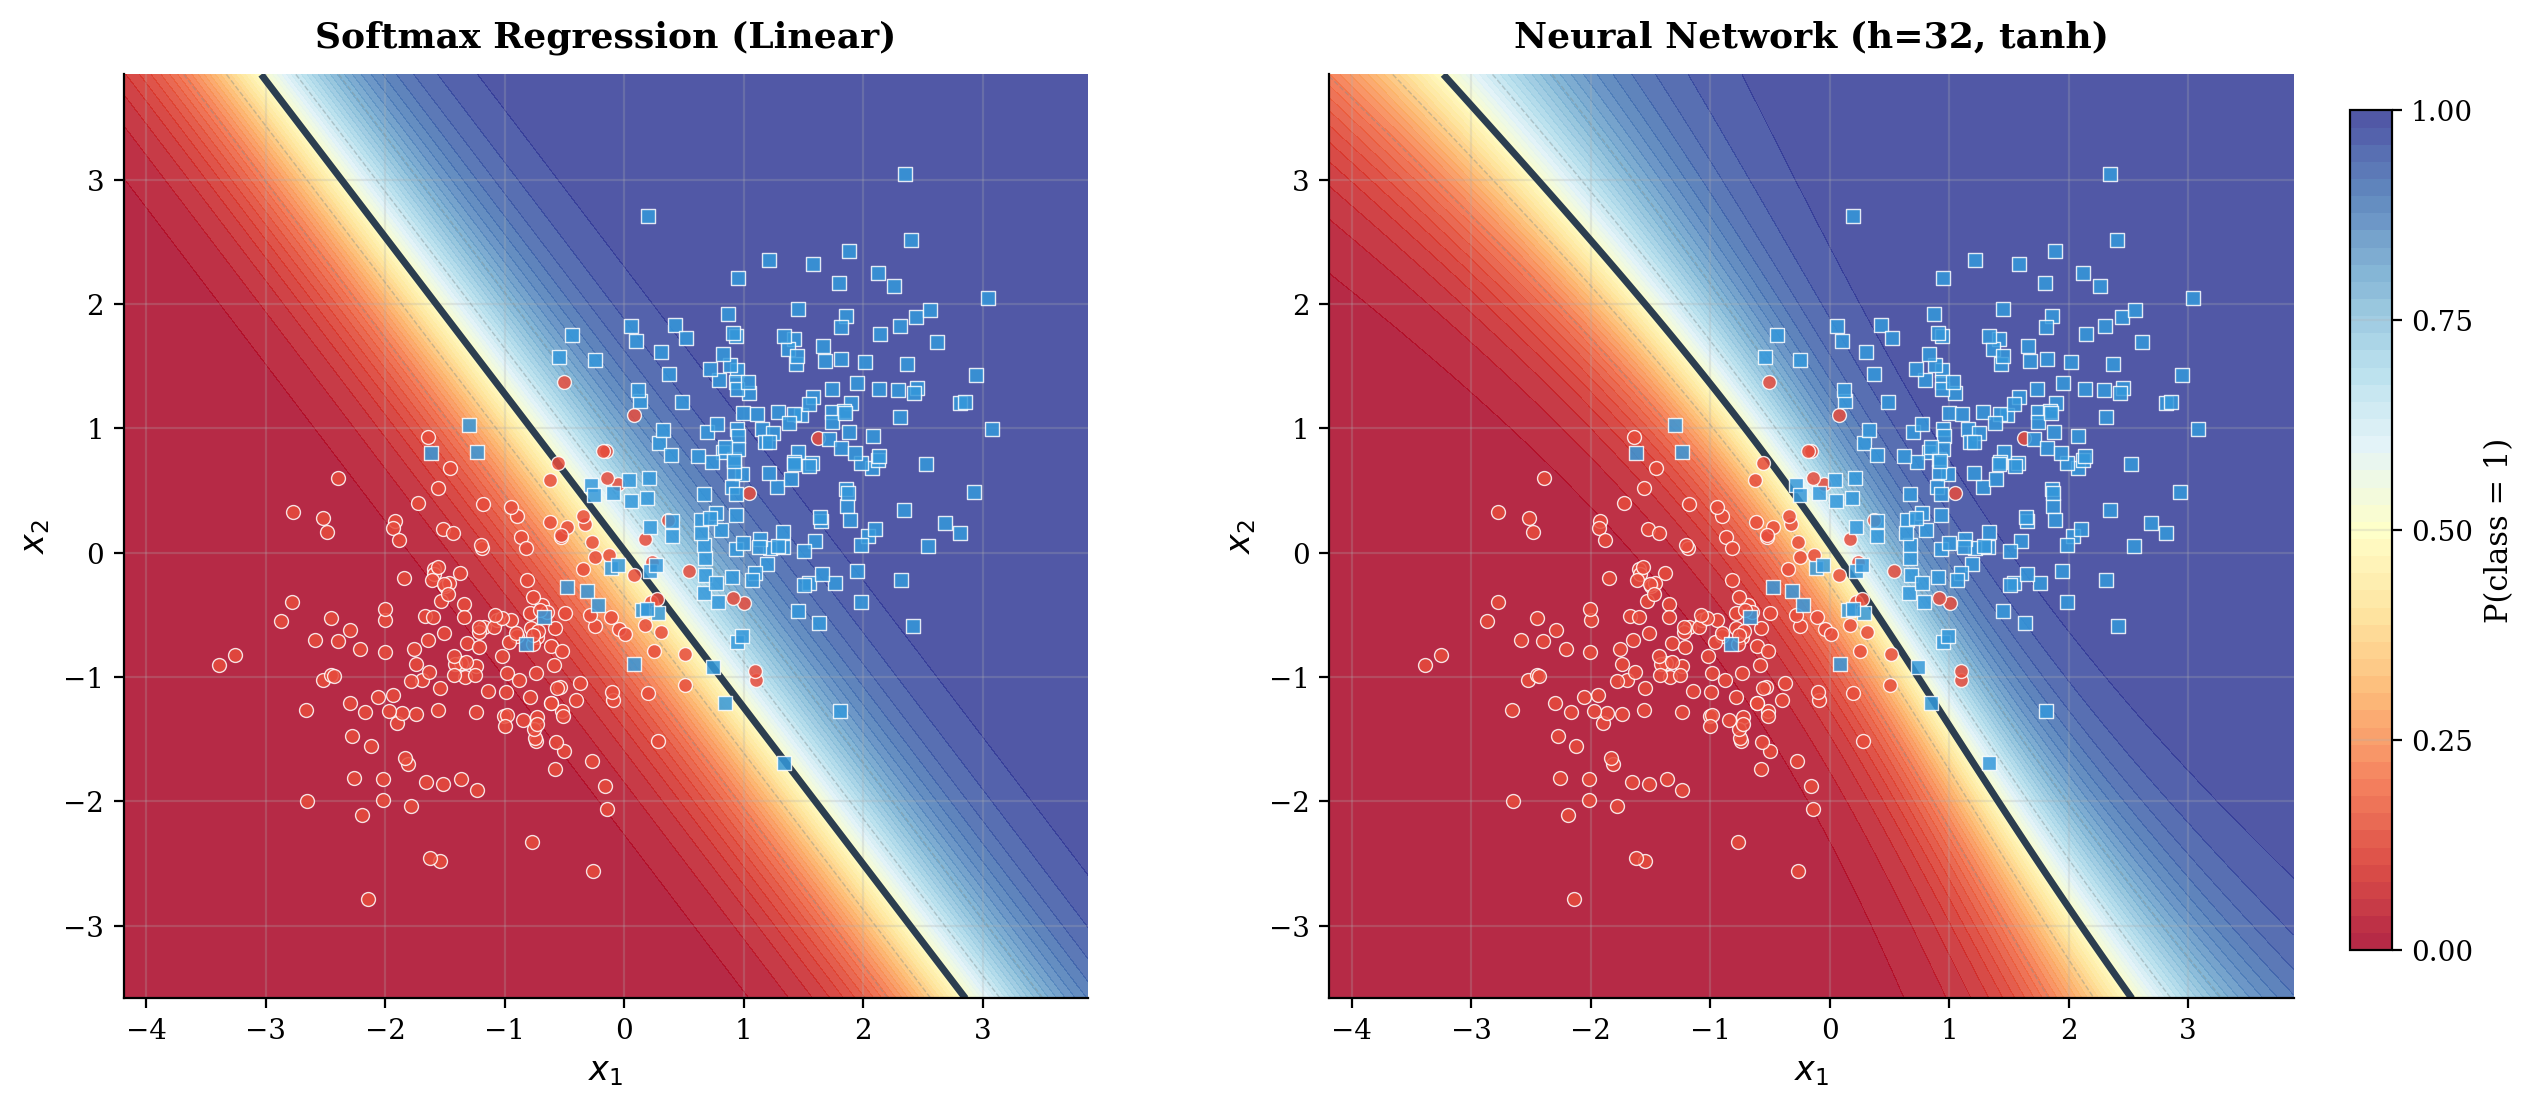
\includegraphics[width=\textwidth]{comparison_lineargaussian.png}
\end{column}
\begin{column}{0.38\textwidth}
\begin{block}{Key Finding}
Bayes-optimal boundary is a hyperplane $\Rightarrow$ \textbf{linear model suffices}.
\end{block}

% \textbf{Mathematical reason:}\\[2pt]
% {\small For shared covariance $\sigma^2 I$, the log-odds are \textit{affine} in $x$:}
% {\small\[
% \log\frac{P(y\!=\!1|x)}{P(y\!=\!0|x)} = \frac{(\mu_1-\mu_0)^\top x}{\sigma^2} + c
% \]}

\begin{itemize}
    \item Both models learn the same boundary
    \item NN's extra parameters are wasted
\end{itemize}

\vspace{0.3em}
\textcolor{softteal}{\textbf{Takeaway:}} Complexity does not justify itself here
\end{column}
\end{columns}

\end{frame}

% ──────────────────────────────────────────
% SLIDE 6: Moons
% ──────────────────────────────────────────
\begin{frame}{Experiment 2: Moons --- Nonlinearity is Essential}

\begin{columns}[c]
\begin{column}{0.60\textwidth}
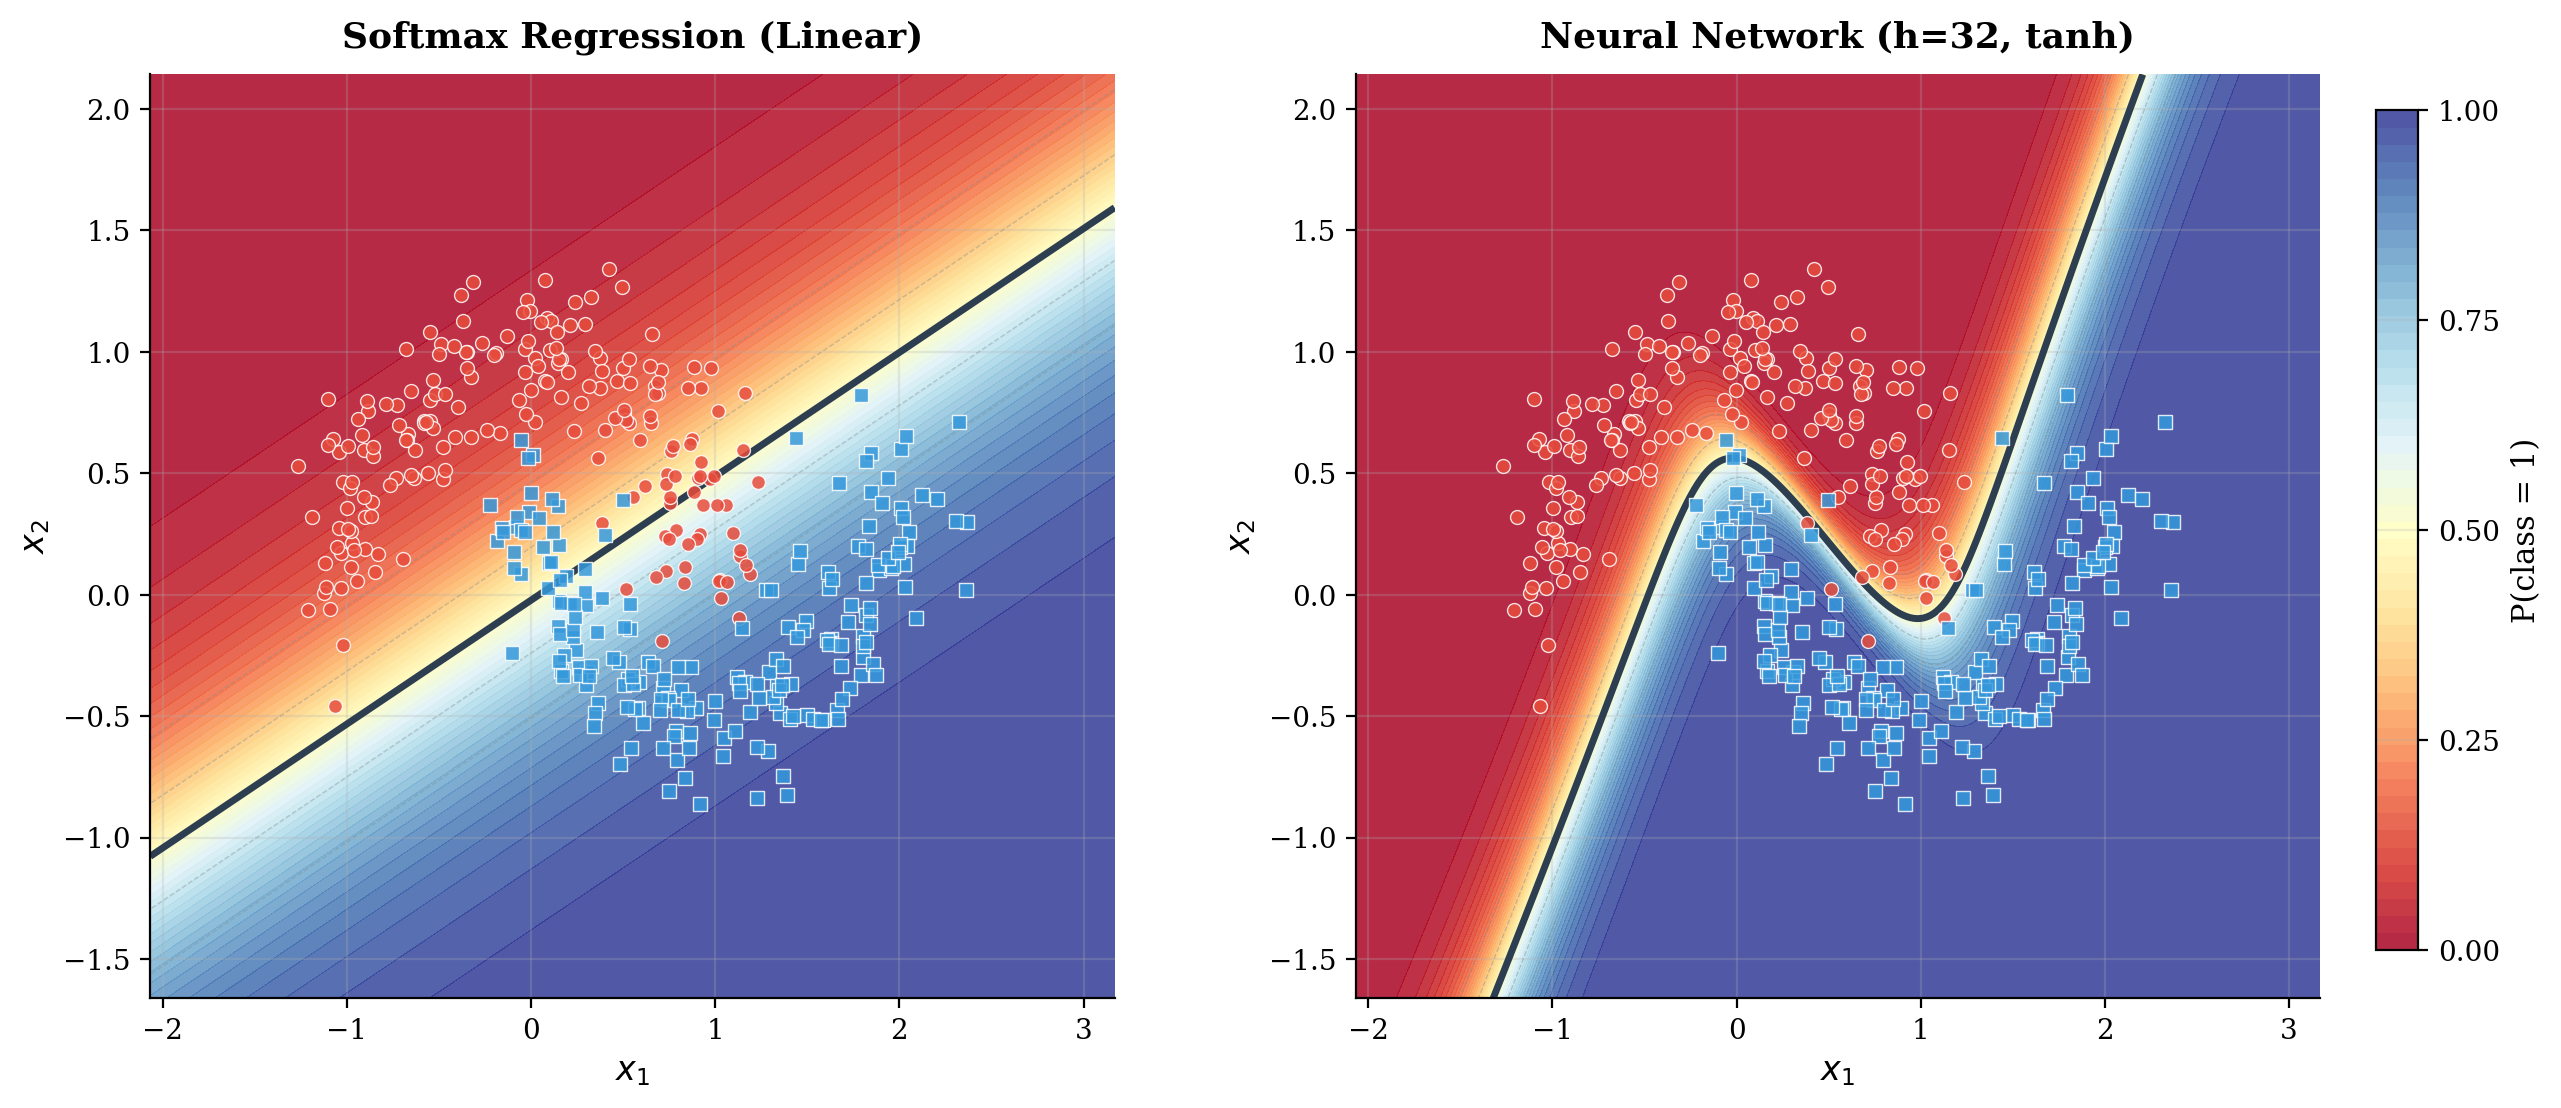
\includegraphics[width=\textwidth]{comparison_moons.png}
\end{column}
\begin{column}{0.38\textwidth}
\begin{block}{Key Finding}
Interleaving arcs are \textbf{not linearly separable} $\Rightarrow$ no hyperplane can separate them.
\end{block}
\begin{itemize}
    \item Softmax places a line through both classes $\Rightarrow$ fails
    \item NN learns a curved boundary $\Rightarrow$ near-100\% accuracy
\end{itemize}

\vspace{0.3em}
\textcolor{softteal}{\textbf{What the hidden layer does:}}\\[2pt]
{\small $h = \tanh(W_1 x + b_1)$ maps $\mathbb{R}^2 \to \mathbb{R}^{32}$.\\ In the new space, the arcs become linearly separable; the output layer draws a hyperplane there.}
\end{column}
\end{columns}

\end{frame}

% ──────────────────────────────────────────
% SLIDE 7: Digits Benchmark
% ──────────────────────────────────────────
\begin{frame}{Experiment 3: Digits Benchmark --- Real-World Task}

\begin{columns}[c]
\begin{column}{0.55\textwidth}
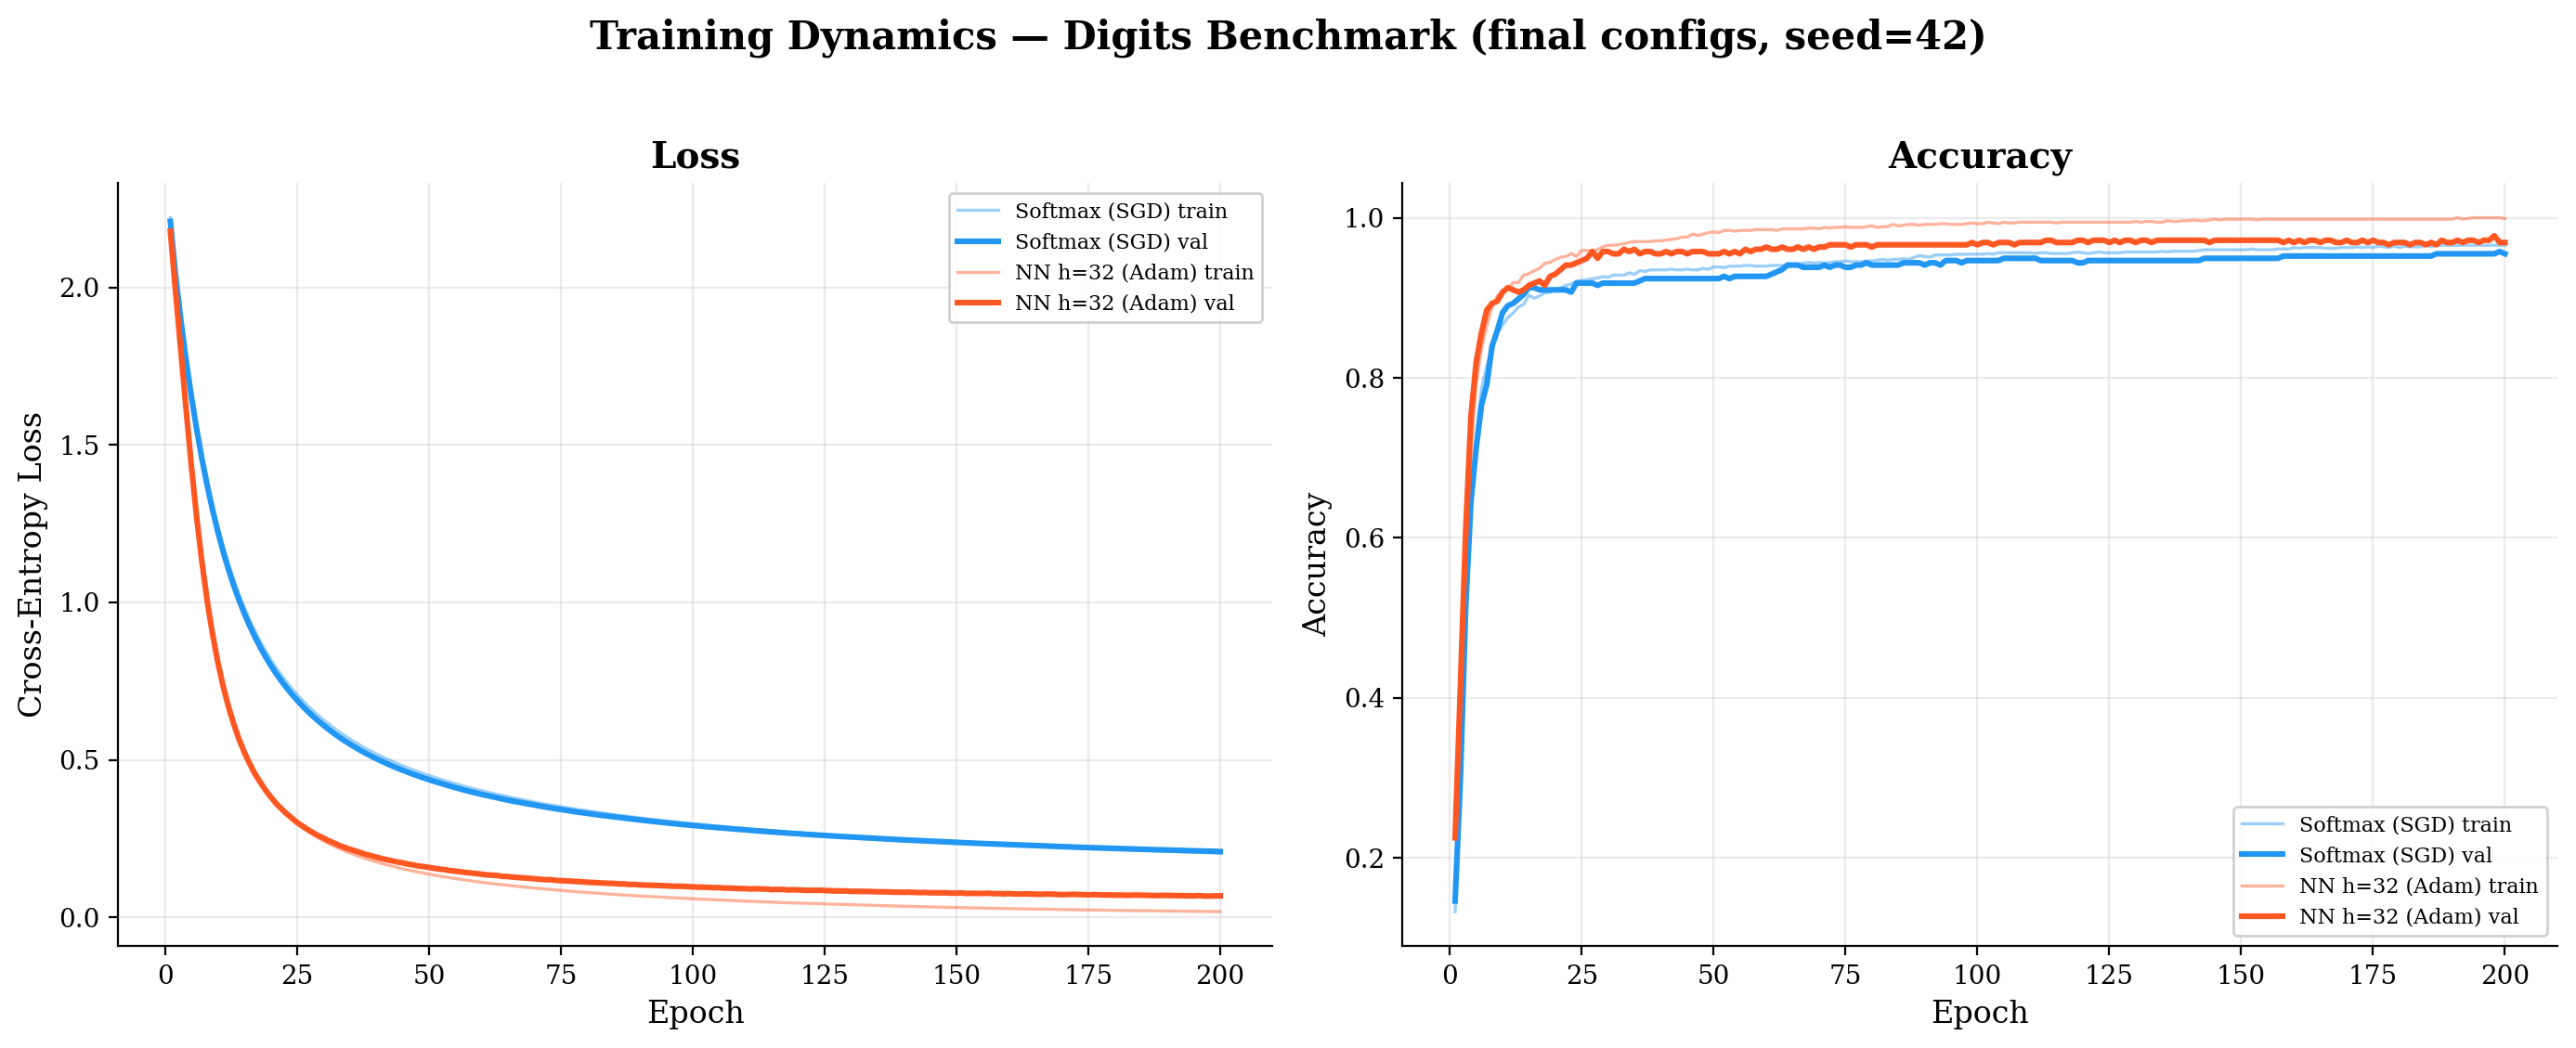
\includegraphics[width=\textwidth]{loss_curves_digits.png}
\end{column}
\begin{column}{0.43\textwidth}
\begin{center}
\begin{tabular}{lcc}
\toprule
\textbf{Model} & \textbf{Acc} & \textbf{CE} \\
\midrule
Softmax & 93.3\% & 0.269 \\
NN $h\!=\!32$ & \textbf{95.7\%} & \textbf{0.157} \\
\bottomrule
\end{tabular}
\end{center}

\vspace{0.5em}
\begin{itemize}
    \item $\sim$2.5 ppt accuracy gain, 42\% lower CE
    \item CE reduction $>$ accuracy gain $\Rightarrow$ NN gives better-calibrated probabilities
    \item Linear model is already strong (93\%)     Digits is ``mostly linear''
\end{itemize}
\end{column}
\end{columns}

\end{frame}

% ──────────────────────────────────────────
% SLIDE 8: Capacity Ablation
% ──────────────────────────────────────────
\begin{frame}{Capacity Ablation: Hidden Width on Moons $\{2, 8, 32\}$}

\begin{columns}[c]
\begin{column}{0.65\textwidth}
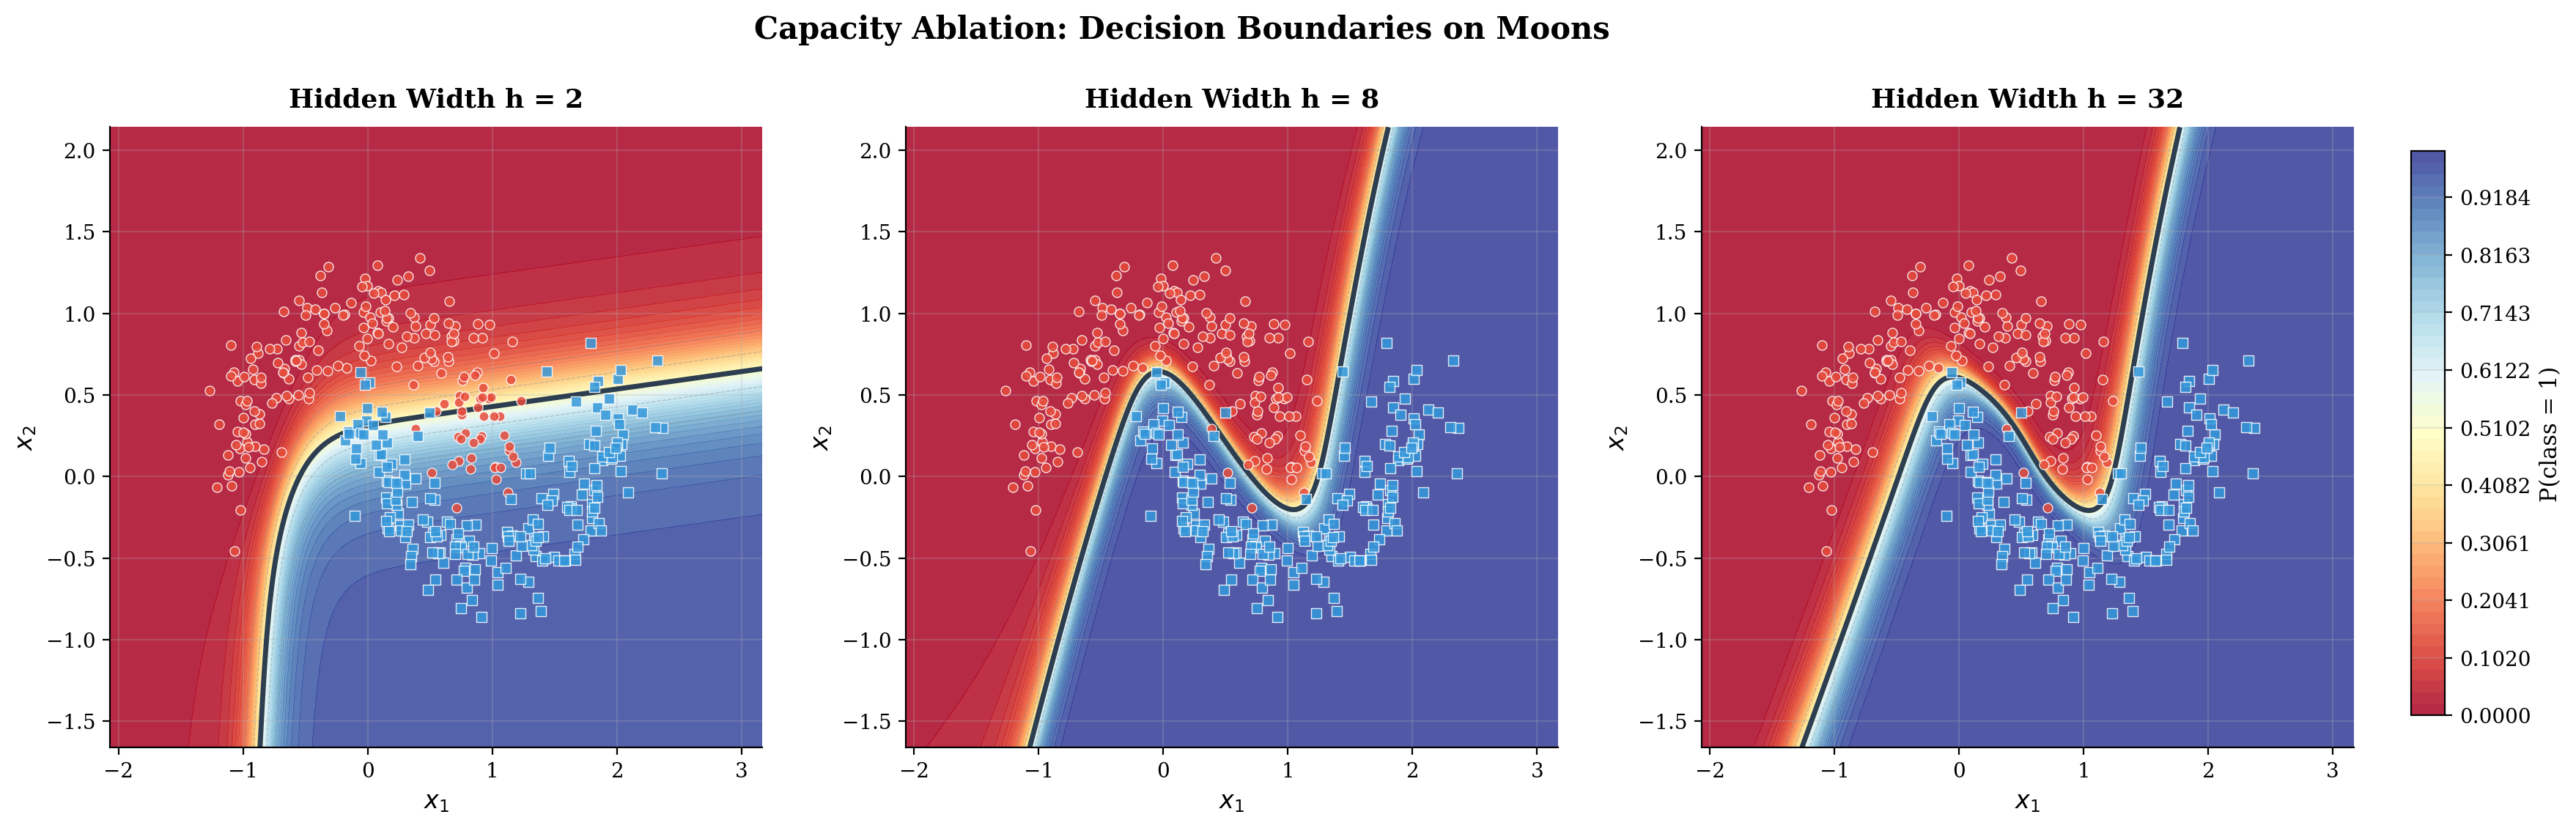
\includegraphics[width=\textwidth]{capacity_ablation_boundaries.png}
\end{column}
\begin{column}{0.33\textwidth}
\begin{itemize}
    \item \textbf{$h\!=\!2$:} crude, nearly linear separation - too few dimensions to represent the curve
    \item \textbf{$h\!=\!8$:} smooth nonlinear boundary captures the moon shape
    \item \textbf{$h\!=\!32$:} no significant difference from $h\!=\!8$
\end{itemize}

\vspace{0.4em}
\textcolor{softteal}{\textbf{Takeaway:}} capacity must match task complexity; beyond that, returns diminish.
\end{column}
\end{columns}

\end{frame}

% ──────────────────────────────────────────
% SLIDE 9: Optimizer Study
% ──────────────────────────────────────────
\begin{frame}{Optimizer Study on Digits (NN $h\!=\!32$, fixed hyperparams)}

\begin{columns}[c]
\begin{column}{0.55\textwidth}
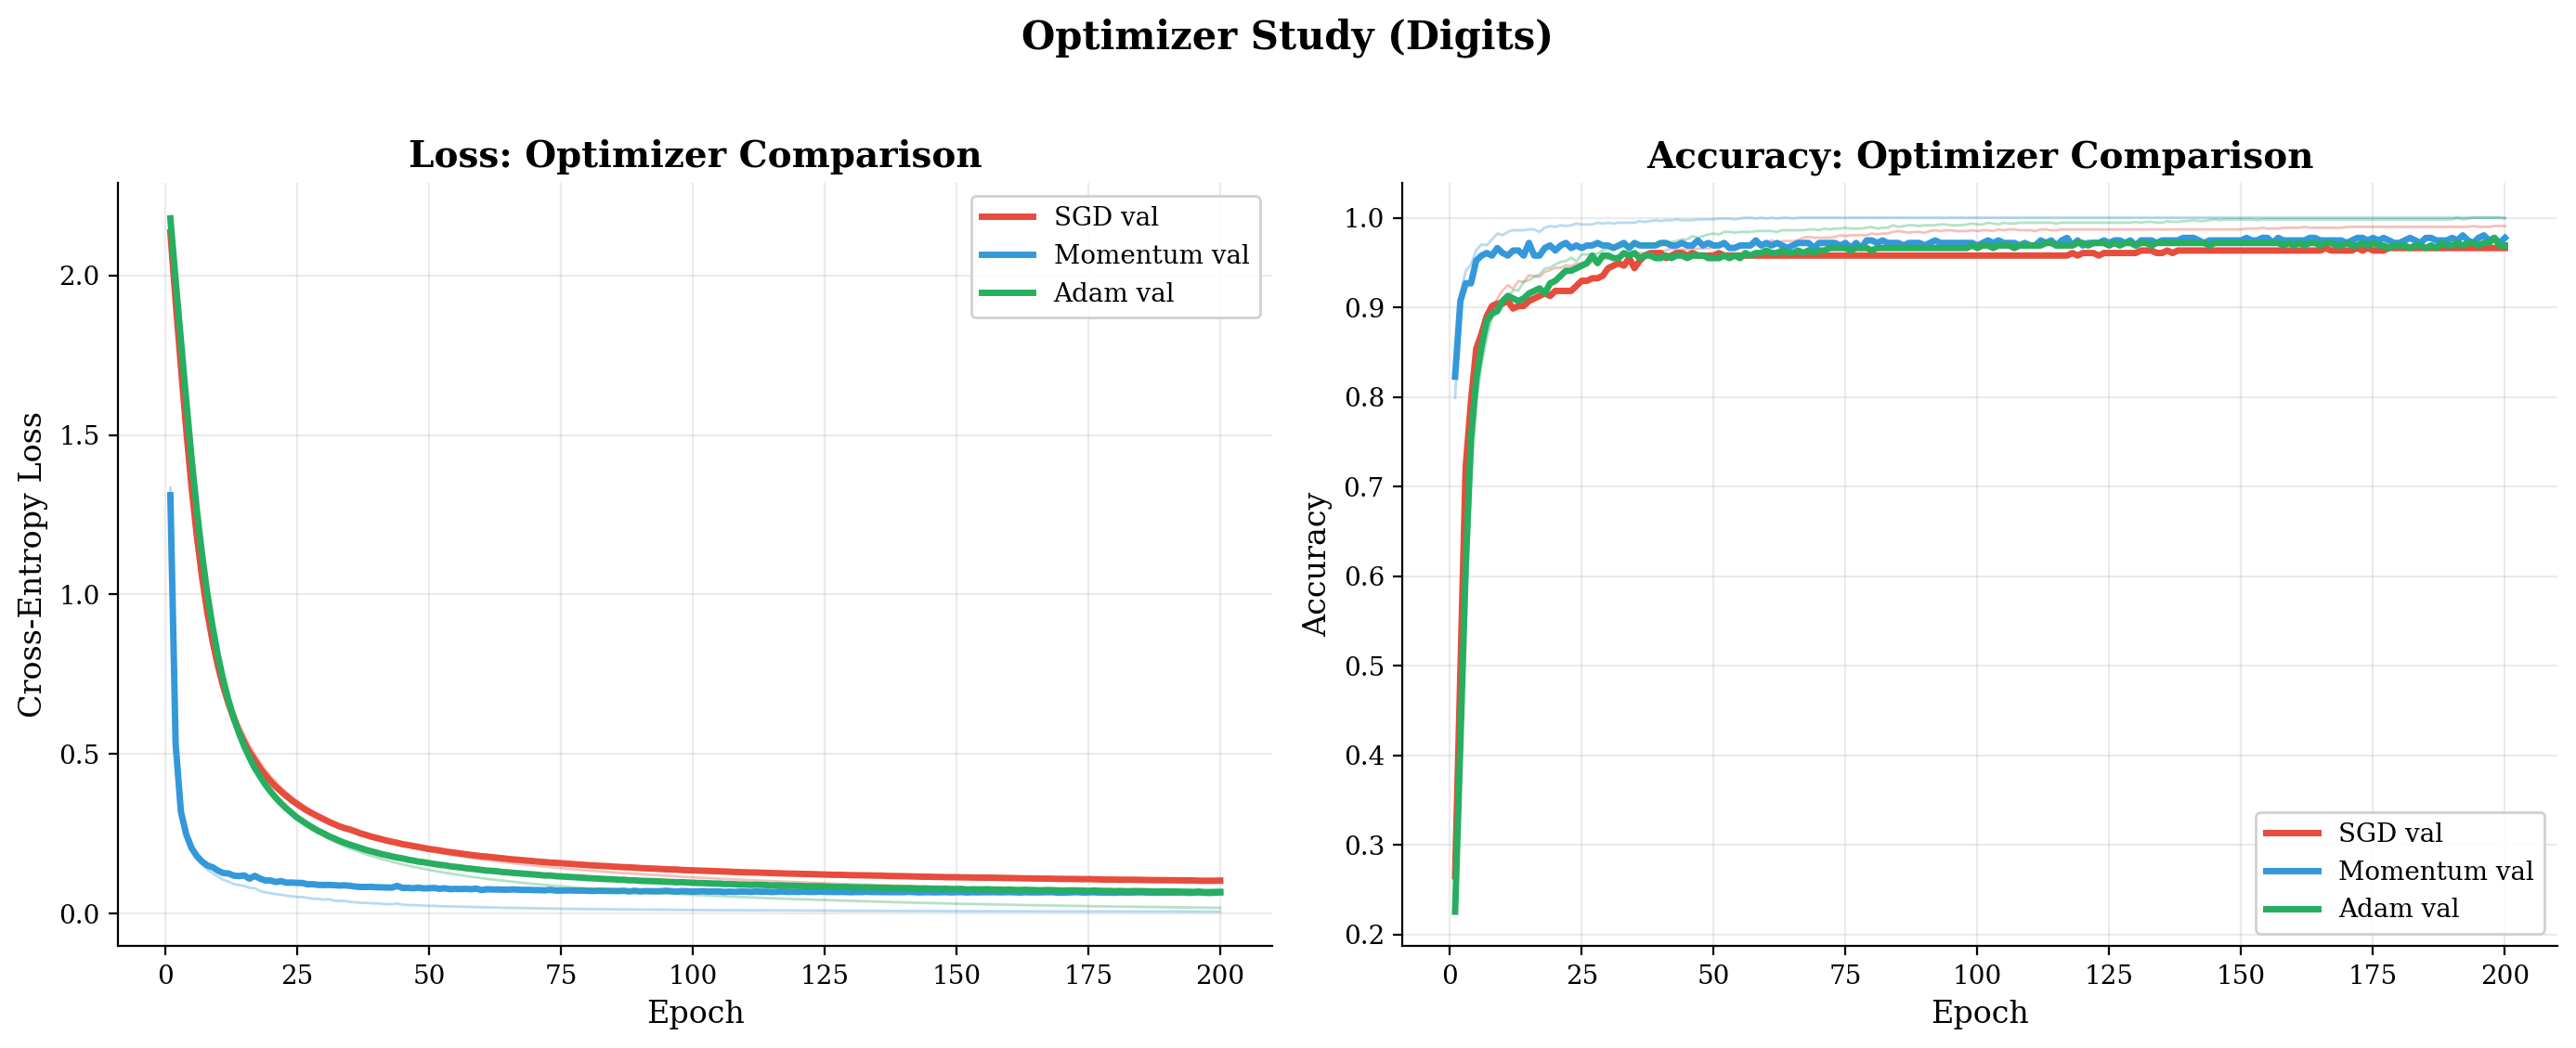
\includegraphics[width=\textwidth]{optimizer_study_digits.png}
\end{column}
\begin{column}{0.43\textwidth}

\begin{tabular}{lccc}
\toprule
\textbf{Optimizer} & \textbf{Acc} & \textbf{CE} & \textbf{Ep.} \\
\midrule
SGD & 94.8\% & 0.170 & 197 \\
Momentum & \textbf{95.4\%} & 0.165 & 197 \\
Adam & 95.1\% & \textbf{0.151} & 197 \\
\bottomrule
\end{tabular}

\vspace{0.5em}
\begin{itemize}
    \item All three reach similar final accuracy ($<$0.6 ppt spread)
    \item Adam: lowest CE (best calibration), fastest early convergence
    \item Momentum: highest accuracy
    \item \textbf{Optimizer choice is secondary to model-class choice} ($\sim$0.5 ppt vs.\ $\sim$2.5 ppt)
\end{itemize}
\end{column}
\end{columns}

\end{frame}

% ──────────────────────────────────────────
% SLIDE 10: Repeated-Seed Evaluation
% ──────────────────────────────────────────
\begin{frame}{Repeated-Seed Evaluation (5 Seeds, 95\% CI)}

\begin{columns}[c]
\begin{column}{0.45\textwidth}
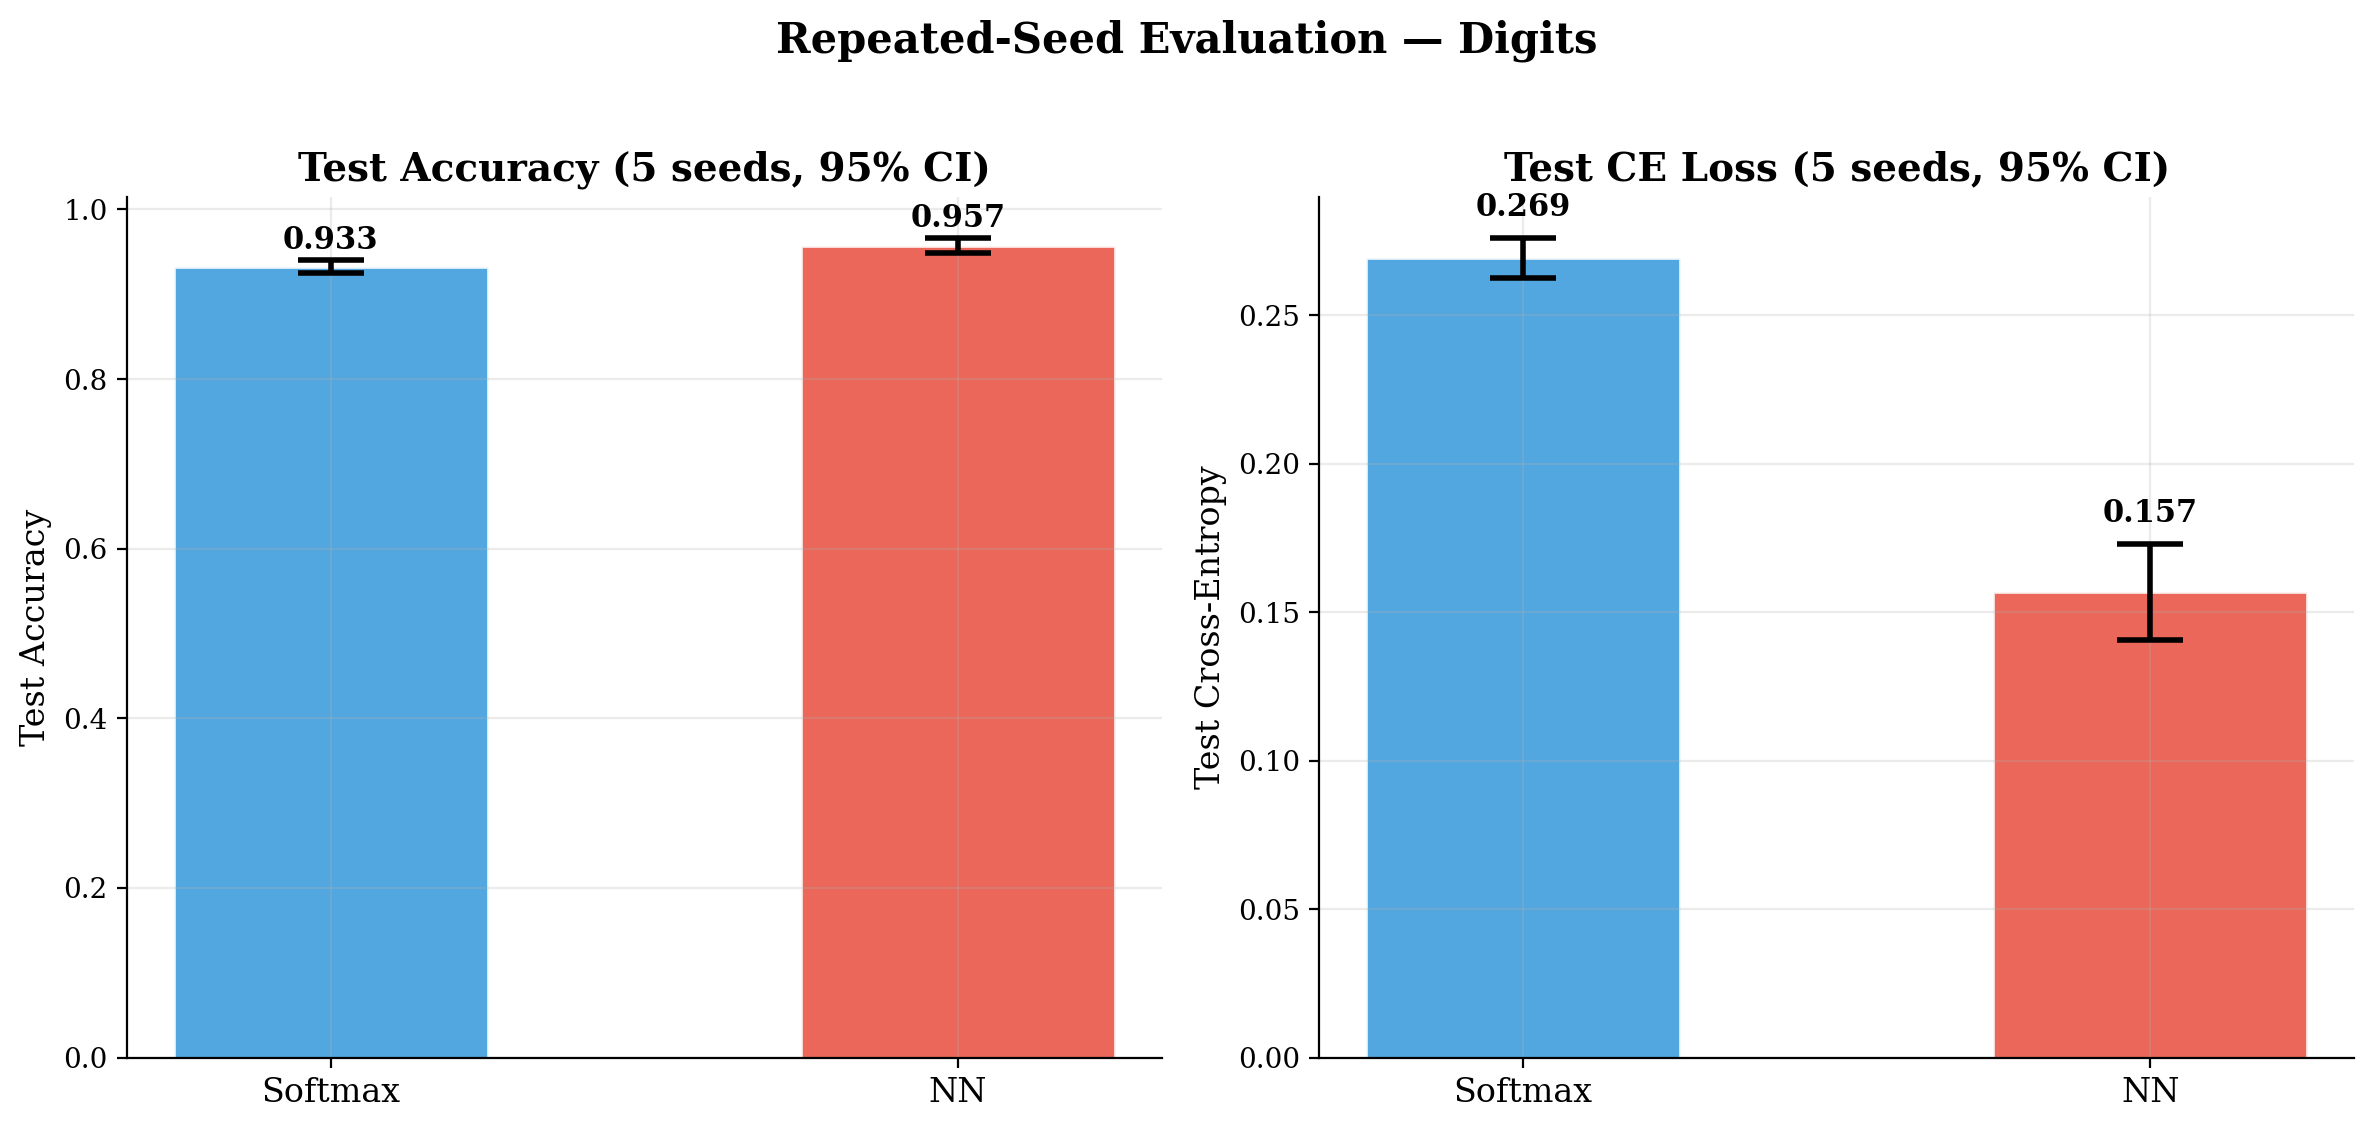
\includegraphics[width=\textwidth]{repeated_seed_digits.png}
\end{column}
\begin{column}{0.53\textwidth}
\[
\bar{x} \pm t_{0.025,\,4} \cdot \frac{s}{\sqrt{5}} = \bar{x} \pm 2.776 \cdot \frac{s}{\sqrt{5}}
\]

\vspace{0.2em}
\begin{tabular}{lcc}
\toprule
& \textbf{Test Accuracy} & \textbf{Test CE} \\
\midrule
Softmax & $93.3\% \pm 0.7\%$ & $0.269 \pm 0.007$ \\
NN & $\mathbf{95.7\% \pm 0.9\%}$ & $\mathbf{0.157 \pm 0.016}$ \\
\bottomrule
\end{tabular}

\vspace{0.4em}
\textcolor{softteal}{\textbf{What repeated seeds add beyond a single run:}}
\begin{itemize}
    \item CIs do not overlap $\Rightarrow$ NN advantage is \textbf{robust}, not a lucky seed
    \item NN has wider CI ($\pm$0.9\% vs.\ $\pm$0.7\%) --- more params $\Rightarrow$ more init sensitivity
    \item Without this, we cannot distinguish genuine model-class gains from random variation
\end{itemize}
\end{column}
\end{columns}

\end{frame}

% ──────────────────────────────────────────
% SLIDE 11: Track A - PCA/SVD
% ──────────────────────────────────────────
\begin{frame}{Track A: PCA/SVD --- How Much Linear Structure Exists?}

\begin{columns}[c]
\begin{column}{0.48\textwidth}
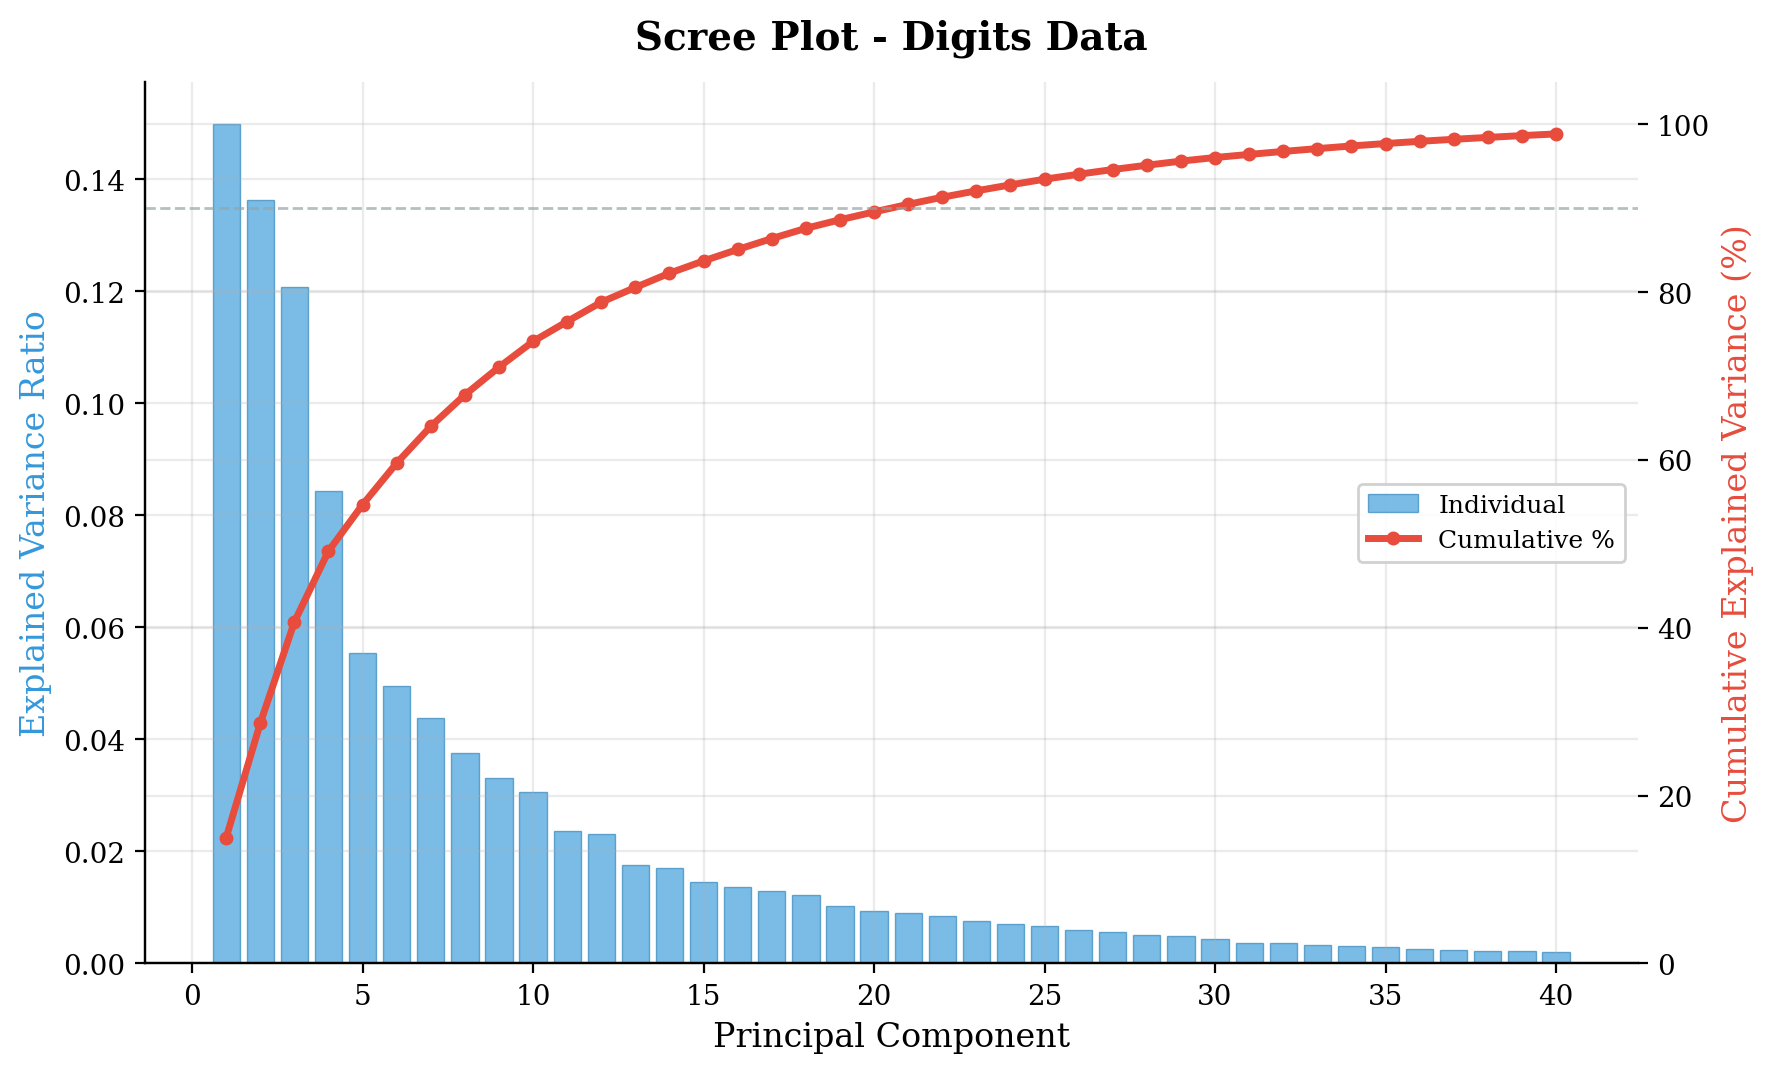
\includegraphics[width=\textwidth]{pca_scree_digits.png}

\vspace{0.2em}
\centering
\small Rapid decay: top 20 PCs capture \textbf{89.6\%} of variance
\end{column}
\begin{column}{0.48\textwidth}
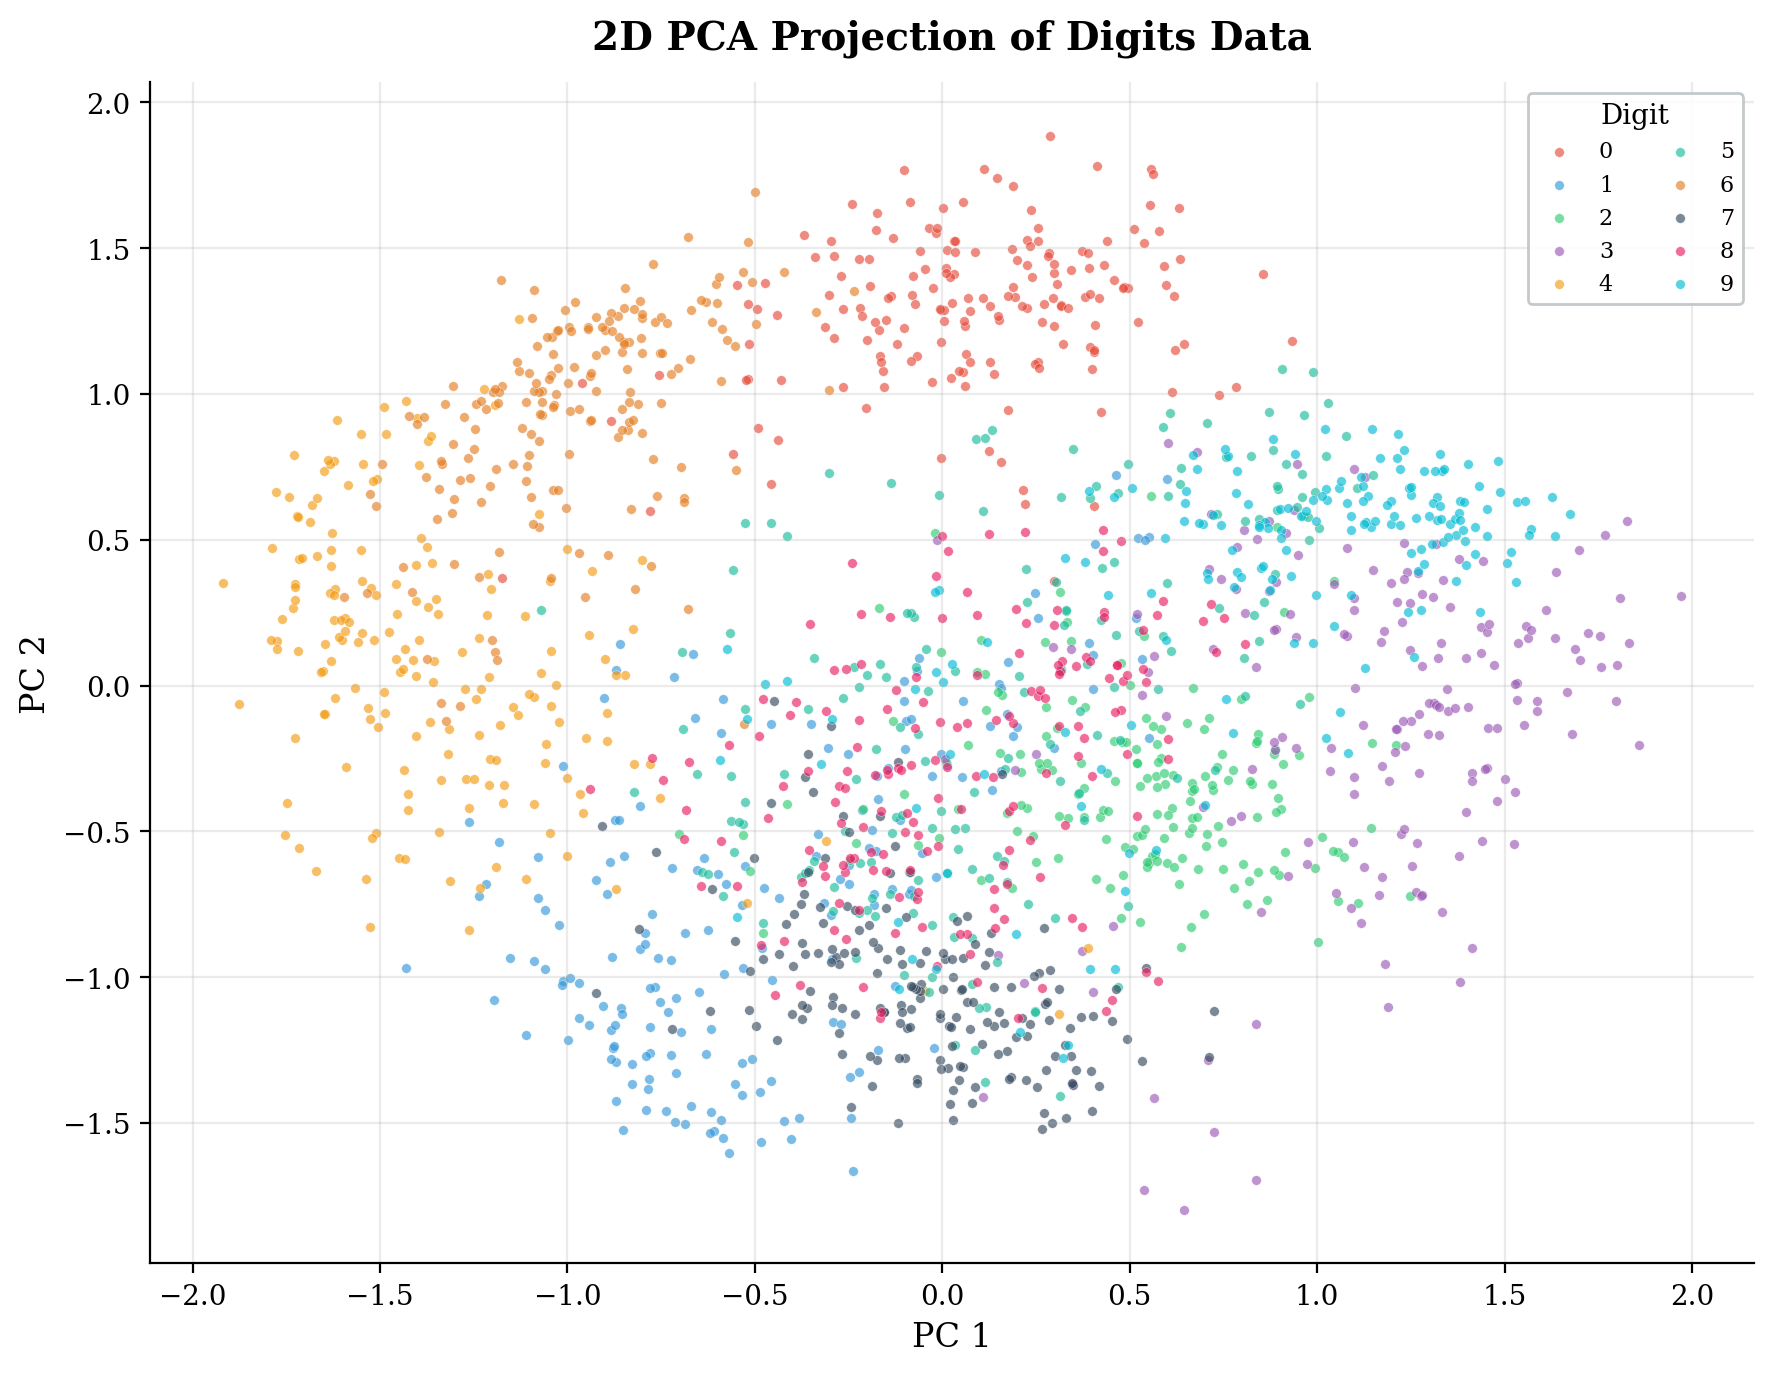
\includegraphics[width=\textwidth]{pca_2d_digits.png}

\vspace{0.2em}
\centering
\small 2D: digits 0,6 separate; 3,5,8 overlap (visual similarity)
\end{column}
\end{columns}

\vspace{0.2em}
\centering
{\small\textcolor{softteal}{\textbf{Key insight:}} The pixel space is effectively ${\sim}$20-dimensional - most variation lives in a low-rank subspace.}

\end{frame}

% ──────────────────────────────────────────
% SLIDE 12: Track A - PCA Softmax Comparison
% ──────────────────────────────────────────
\begin{frame}{Track A: Softmax Performance vs.\ PCA Dimensions}

\begin{columns}[c]
\begin{column}{0.55\textwidth}
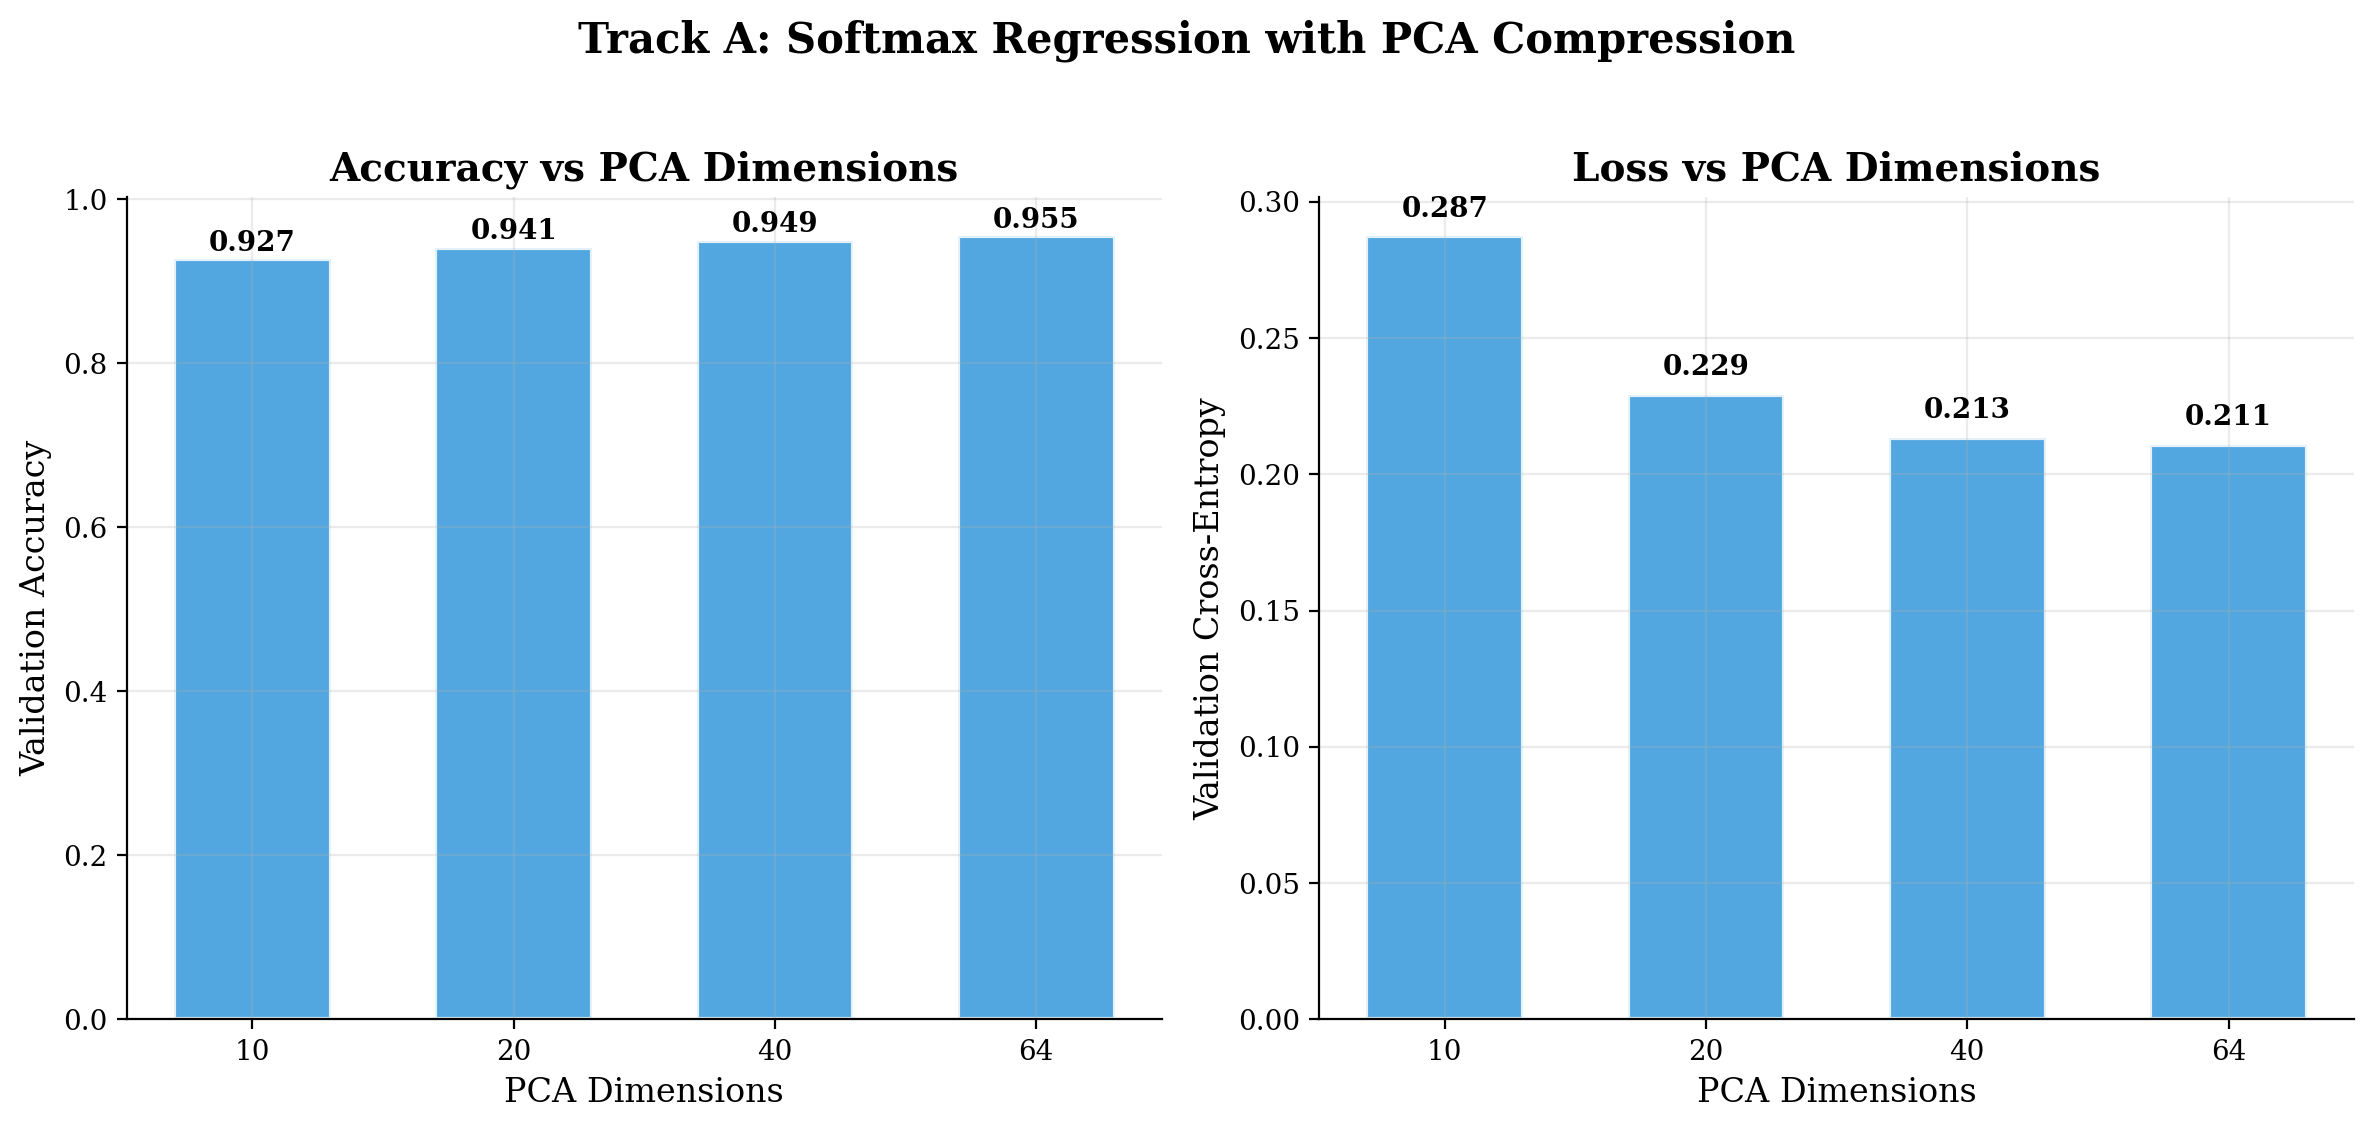
\includegraphics[width=\textwidth]{pca_softmax_comparison.png}
\end{column}
\begin{column}{0.43\textwidth}
\begin{tabular}{ccc}
\toprule
\textbf{PCA $m$} & \textbf{Val Acc} & \textbf{Val CE} \\
\midrule
10 & 92.7\% & 0.287 \\
20 & 94.1\% & 0.229 \\
40 & 94.9\% & 0.213 \\
64 (full) & 95.5\% & 0.211 \\
\bottomrule
\end{tabular}

\vspace{0.5em}
\begin{itemize}
    \item $m{=}20$: discard 69\% of dims, lose only 1.4 ppt
    \item Digits is ``mostly linear'' - linear methods already capture most discriminative structure
    \item NN at full 64 dims (95.7\%) still beats Softmax at any PCA level $\Rightarrow$ \textbf{nonlinear features add value beyond what PCA captures}
\end{itemize}
\end{column}
\end{columns}

\end{frame}

% ──────────────────────────────────────────
% SLIDE 13: Failure Case
% ──────────────────────────────────────────
\begin{frame}{Failure Case: Under-Capacity NN ($h\!=\!2$) on 10-Class Digits}

\begin{columns}[c]
\begin{column}{0.55\textwidth}
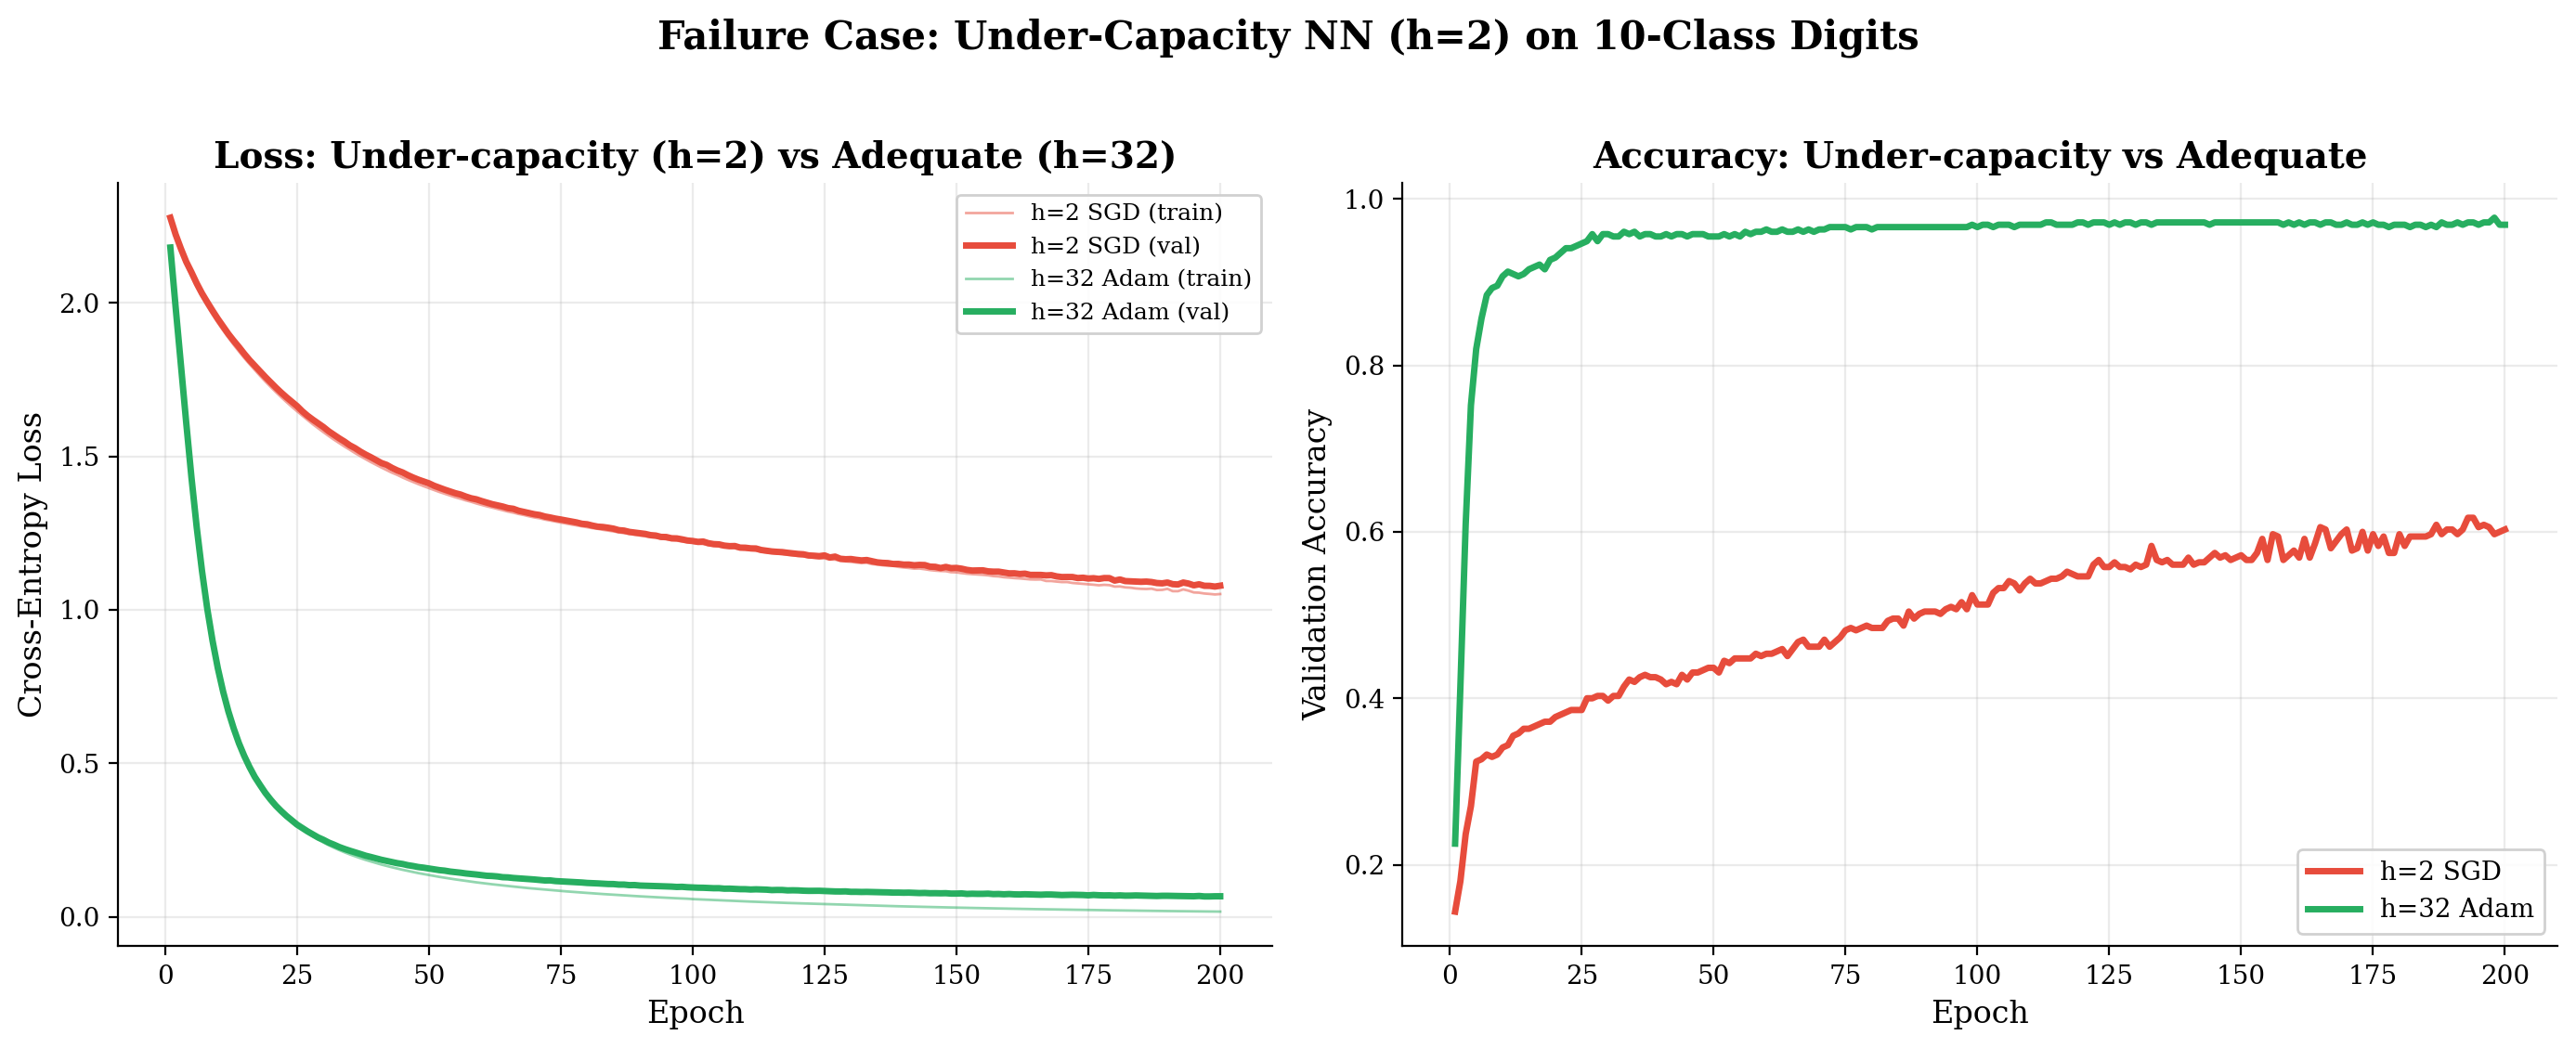
\includegraphics[width=\textwidth]{failure_analysis.png}
\end{column}
\begin{column}{0.43\textwidth}

{\small
\begin{tabular}{lcc}
\toprule
& \textbf{Acc} & \textbf{CE} \\
\midrule
Softmax (linear) & 93.3\% & 0.269 \\
NN $h\!=\!2$ & \textcolor{accentred}{59.0\%} & \textcolor{accentred}{1.113} \\
NN $h\!=\!32$ & 95.7\% & 0.157 \\
\bottomrule
\end{tabular}
}

\vspace{0.3em}
{\small\textbf{Why it fails: capacity, not optimisation:}}
\begin{itemize}\itemsep0.1em
    \item {\small 2-D bottleneck \textbf{destroys} 64-D information}
    \item {\small Same optimizer \& epochs as $h{=}32$ $\Rightarrow$ not optimizer}
    \item {\small Train + val loss stay high $\Rightarrow$ \textbf{underfitting}}
    \item {\small \textcolor{softteal}{\textbf{Lesson:}} Capacity must match task complexity before optimisation can help.}
\end{itemize}
\end{column}
\end{columns}

\end{frame}

% ──────────────────────────────────────────
% SLIDE 14: Discussion (Q1-Q2)
% ──────────────────────────────────────────
% SLIDE 14: Core Questions
% ──────────────────────────────────────────
\begin{frame}{Answering the Core Questions}
\small
\begin{itemize}\itemsep0.8em
    \item \textcolor{softteal}{\textbf{Q1: When is the linear model geometrically sufficient?}} \\
    When the true data boundary is flat (Gaussian), but it fails when boundaries must curve (Moons).

    \item \textcolor{softteal}{\textbf{Q2: What representational change does the hidden layer provide?}} \\
    It learns a nonlinear transformation that ``untwists'' complex data into a linearly separable space.

    \item \textcolor{softteal}{\textbf{Q3: When does additional complexity fail to justify itself?}} \\
    When the simple baseline already captures the geometry, or if the capacity is severely bottlenecked.

    \item \textcolor{softteal}{\textbf{Q4: What does the failure case teach us?}} \\
    It demonstrates that representational capacity is a strict prerequisite that optimisation cannot substitute.

    \item \textcolor{softteal}{\textbf{Q5: What do repeated-seed statistics add beyond a single run?}} \\
    They prove that the neural network's advantage is robust across random initialisations, not just a lucky artefact.
\end{itemize}

\end{frame}

% ──────────────────────────────────────────
% SLIDE 15: Limitations
% ──────────────────────────────────────────
\begin{frame}{Limitations --- What Our Study Does Not Show}

\begin{itemize}
    \item \textbf{Architecture constraint}: Single hidden layer, $\tanh$ only --- deeper networks or ReLU may behave differently.
    \item \textbf{Data scale}: Small-scale data (${\sim}1{,}800$ samples, $d{=}64$) --- conclusions may not transfer to ImageNet-scale tasks.
    \item \textbf{Regularisation}: Only $L_2$ regularisation ($\lambda{=}10^{-4}$); no dropout, batch norm, or cross-validation.
    \item \textbf{Statistical limits}: 5 seeds assume approximate normality; optimizers were tested at one fixed setting.
\end{itemize}

\vspace{0.5em}
Our findings reliably characterise this specific comparison on these three tasks under this fixed protocol.

\end{frame}

% ──────────────────────────────────────────
% SLIDE 16: Summary
% ──────────────────────────────────────────
\begin{frame}{Summary of Key Findings}

\begin{center}
\begin{tabular}{@{}lp{5.5cm}p{5.5cm}@{}}
\toprule
\textbf{Task} & \textbf{Linear model} & \textbf{Hidden layer} \\
\midrule
Gaussian & \textcolor{accentgreen}{Sufficient}; Bayes boundary is a hyperplane & No benefit; wasted parameters \\[4pt]
Moons & \textcolor{accentred}{Fails}; cannot separate curved arcs & \textcolor{accentgreen}{Essential}; learns nonlinear coordinate change \\[4pt]
Digits & \textcolor{accentgreen}{Strong} (93.3\%); mostly linear structure & \textcolor{accentgreen}{Modest gain} (95.7\%); captures residual nonlinear features \\[4pt]
Digits $h{=}2$ & \textcolor{accentgreen}{93.3\%};  better! & \textcolor{accentred}{59.0\%}; bottleneck destroys information \\
\bottomrule
\end{tabular}
\end{center}

\vspace{0.4em}

\end{frame}

% ──────────────────────────────────────────
% SLIDE 17: Thank You
% ──────────────────────────────────────────
\begin{frame}{}

\vfill
\centering
{\LARGE \textbf{Thank You}}

\vspace{1em}
{\large Questions?}

\vspace{2em}
\vfill

\end{frame}

\end{document}
